\documentclass[11pt,a4paper]{article}
\usepackage[light,math]{iwona}
\usepackage[usenames,dvipsnames]{color}
\usepackage{tikz}
\usepackage{graphicx}
\usepackage{hyperref}
\usetikzlibrary{calc,shapes,arrows,automata,trees,shadows,decorations.pathmorphing,positioning, shapes.misc,shapes.arrows,chains,matrix,scopes,decorations.pathmorphing,backgrounds}
\newcommand{\HRule}{\rule{\linewidth}{0.5mm}}

\begin{document}
%
\begin{titlepage}
\begin{center}
% Upper part of the page


\textsc{\color{Sepia}{\LARGE CS~434}}\\[1.5cm]
\textsc{\Large Week~Two}\\[0.5cm]
%graphic
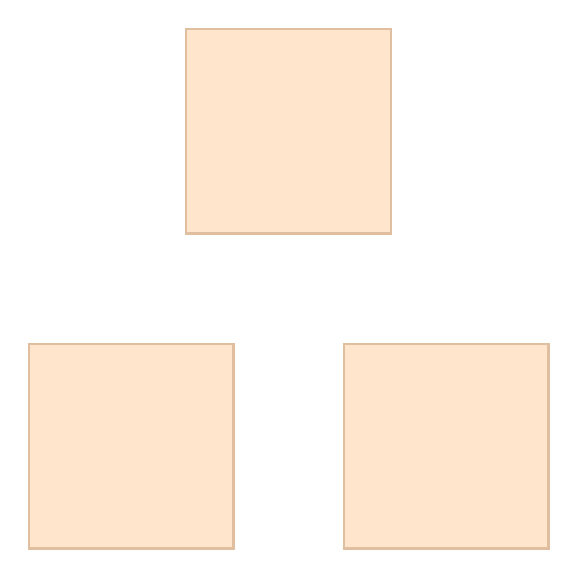
\begin{tikzpicture}
  [inner sep=13mm, place/.style={circle,draw=blue!50,fill=blue!20,thick},
   transition/.style={rectangle,draw=brown!50,fill=orange!20,thick}]
\node at ( 0,0) [transition] {};
  \node at ( 2,  -4) [transition] {};
  \node at (-2, -4) [transition] {};
\end{tikzpicture}
% Title
\HRule \\[0.4cm]
{ \huge \bfseries O O Programming Java}\\[0.4cm]
\HRule \\[1.5cm]


% Author and supervisor
\begin{minipage}{0.4\textwidth}
\begin{flushleft} \large
\emph{Author:}\\
Jason \textsc{Mansfield}
\end{flushleft}
\end{minipage}
\begin{minipage}{0.4\textwidth}
\begin{flushright} \large
\emph{Instructor:} \\
Hong \textsc{Zhu}
\end{flushright}
\end{minipage}
\vfill
% Bottom of the page
{\large \today}
\end{center}
\end{titlepage}
\tableofcontents
\section{Actors}
\section{Stakeholders and Interests}
\section{Preconditions}
\section{Success Guaranteed}
\section{Main Success Scenario}
\subsection{}
\subsection{}
\section{Extensions}
\subsection{}
\subsection{}
\section{Special Requirements}
\section{Technology and Data Variation List}
\section{Frequency of Occurrence}
\section{Open Issues}

\end{document}